
\newcommand{\fidel}{\mathscr{F}}
\newcommand{\tracedist}{\mathscr{T}}
\newcommand{\trotterchan}[2]{{S_{#1}{\parens{ #2 }}}}
\newcommand{\tschan}[2]{\mathcal{T}^{#1}{( #2 )}}
    
\newcommand{\achan}[1]{\mathcal{T}_{A}^{2k}{( #1 )}}
\newcommand{\bchan}[1]{\mathcal{Q}_{B}{( #1 )}}
 
\newcommand{\evolchan}[1]{\mathcal{U}{ ( #1 ) }}
\newcommand{\specnorm}[1]{\left| \left| #1 \right| \right|_\infty}
\newcommand{\liouv}{\mathcal{L}}
\newcommand{\prodform}{S_{2k}}
\newcommand{\indone}[1]{\norm{ #1 }_{1\rightarrow 1}}
\newcommand{\indonedef}[1]{\max_{\rho : \norm{\rho}=1} \norm{ #1 }_1}
    


\chapter{Numerics}


\section{Composite Simulations} \label{sec:numerical_sim}
In this section we highlight the details of configuring our numerical investigations by defining Hamiltonians of interest. We then discuss partitioning strategies and choice of an error measure before presenting numerical results. The choice of error measure usually does not require a dedicated subsection. However, when considering composite algorithms, there is a subtle feature in that not all algorithms may be treated on equal footing by the same error measure, which can lead to inconsistencies. For our purposes, the trace distance is the most useful measure of choice. Rather than computing upper-bounds, the numerical results we provide here are exact calculations of the cost $C$, or the precise counts on the number of quantum gates with the form $e^{-i\frac{t}{r} \bigotimes_j \sigma_j^\nu}$ required to meet some desired precision $\epsilon$. We write gates in this form to highlight that the Hamiltonian summands in our simulations are always written as a tensor product of Pauli operators, allowing for a nice parallel to the well known rotation gates in the context of quantum computing. For imaginary time, although this form still holds in our numerics, the same analogy does not hold, as we are simply constructing $e^{-\frac{\beta}{r} H_j}$ on a classical computer which can be of somewhat arbitrary form. 

In order to calculate $C$, we have constructed a library to compile any desired product formula simulation, given a list of Hamiltonian terms, partition, QDrift samples, simulation time and desired precision. These simulator objects are handled by external functions that can partition the simulators, calculate errors and exact costs, or approximate simulation cost via Monte-Carlo methods and more. The library is built on NumPy, but also contains conversion functions to load Hamiltonians generated by quantum chemistry packages OpenFermion \cite{mcclean2020openfermion} and PySCF \cite{sun2018pyscf} to simulate systems of interest. It also contains methods for geometrically local simulations to compute blockings using the required set logic.

\subsection{Hamiltonians of Interest}
Within this section, we introduce the Hamiltonians in our numerical investigation of composite algorithms, as well as briefly outline methods used for their generation. 

\subsubsection{Electronic Structure Hamiltonians in Second Quantization} \label{sec:hydrogen} The electronic structure problem is perhaps one of the most famous classically intractable problems that has vast applications in quantum chemistry. In order to write down these Hamiltonians, it is first necessary to introduce Fermionic creation and annihilation operators. Fermions are particles with half-integer spin that obey Fermi-Dirac statistics, meaning they obey the following anti-commutation relations:
\begin{align}
    \{a_m, a_n^\dagger\}:&= a_ma_n^\dagger + a_n^\dagger a_m = \delta_{mn} \\
    \{a_m, a_n\} &= \{a_m^\dagger, a_n^\dagger\} = 0
\end{align}

We work in Fock space where the subscripts of operators indicate the excitation number or the atomic orbital of an electron. Molecular electronic structure Hamiltonians then take the following form: 
\begin{equation}\label{eq:secondquant}
    H = \sum_{mn} h_{mn} a_m a_n^\dagger + \sum_{pqrs} h_{pqrs} a_p a_q a_r^\dagger a_s^\dagger 
\end{equation} 
Here the first term represents single excitations and the second term keeps track of double excitations or ``hopping" amongst orbitals. The coefficients $h$ are molecular integrals that depend on the basis of choice to describe the molecule \cite{whitfield2011simulation}. Further, more can be done to aid in the implementation of this problem on a quantum computer. The Jordan-Wigner transformation provides a one-to-one mapping between the fermionic and spin operators. This will allow us to write down the time evolution operator in terms of the universal rotation gates (and CNOT gates). To understand the transformation, first observe: 
\begin{align}
    a^\dagger &= \begin{bmatrix}
    0 & 0\\
    1 & 0 
    \end{bmatrix} = \frac{\sigma^x - i\sigma^y }{2}:= \sigma^- \\
    a &= \begin{bmatrix}
    0 & 1\\
    0 & 0 
    \end{bmatrix} = \frac{\sigma^x + i\sigma^y }{2}:= \sigma^+
\end{align}
Now to build in the desired commutation relations and  generalize this to a Hilbert space for $N$ qubits, or the tensor (Kronecker) product of $N$ 2-dimensional Hilbert spaces $\hilbSpace = \bigotimes_{i=1}^N \hilbSpace_i$:

\begin{align}
    a_n^\dagger & \Leftrightarrow \openone^{\otimes n -1} \otimes  \sigma^- \otimes (\sigma^z)^{\otimes N- n -1} \\
    a_n & \Leftrightarrow \openone^{\otimes n -1} \otimes  \sigma^+ \otimes (\sigma^z)^{\otimes N- n -1}
\end{align}

In order to build these Hamiltonians numerically, we use the OpenFermion \cite{mcclean2020openfermion} and PySCF \cite{sun2018pyscf} packages for quantum chemistry. OpenFermion is a library that allows for the easy manipulation of fermionic operators that arise in quantum chemistry, as well as it interfaces with a variety of electronic structure packages that perform molecular integrals in the basis of choice to generate Hamiltonians in the form of Equation \ref{eq:secondquant}. Further, OpenFermion also has the Jordan Wigner transform built in, allowing one to construct this Hamiltonian in the Pauli basis. PySCF was our electronic structure package of choice to compute molecular integrals. \\

Given the form of Equation \ref{eq:secondquant}, we observe that our Hilbert space needs to be truncated. An active space calculation does exactly this; the Hamiltonian is written in a space such that only so many orbitals are ``active" or such that an electron can be excited to occupy active orbitals. We generate all of our electronic structure Hamiltonians in the minimal basis where we use a the number of qubits equal to the total period of the molecule. For our numerical investigation, we provide a function to generate chains of hydrogen atoms given a very simple input; bond length and number of atoms. The function uses PySCF to compute the molecular integrals, and then uses the data to build the Hamiltonian in an active space implied by the minimal basis, and using a minimal spin configuration. 

\subsubsection{Jellium Uniform Electron Gas}
Jellium is a model of a uniform electron gas that captures the interactions between delocalized electrons in a solid with uniformly distributed positive potentials serving as Nuclei. It is not only a system of interest in Materials Science, but also as a benchmark system in quantum simulation. More compact representations of this Hamiltonian have been proposed as a candidate for experimental simulation on near-term hardware \cite{babbush2018low}. The system Hamiltonian has a closed form representation and does not require any additional molecular integrals to construct:
\begin{equation}
    H = \frac{1}{2} \sum_{p, \sigma} k^2_p a^\dagger_{p, \sigma} a_{p, \sigma} - \frac{4\pi}{\Omega}\sum_{p\neq q, j, \sigma} \parens{\zeta_j \frac{e^{ik_{q-p} \cdot R_j}}{k^2_{p-q}}} a^\dagger_{p, \sigma} a_{q, \sigma} + \frac{2\pi}{\Omega} \sum_{(p,\sigma)\neq (q, \sigma '), \nu \neq 0} \frac{a^\dagger_{p, \sigma} a^\dagger_{q, \sigma '} a_{q+\nu, \sigma '} a_{p -\nu, \sigma}}{k_\nu^2}
\end{equation}
where the $j$th nuclei has position $R_j$ and atomic number $\zeta_j$, and $k_\nu=\frac{2\pi \nu}{\Omega^{\frac{1}{3}}}$ with cell volume $\Omega$ and $\sigma$ containing both up and down spins. For the derivation of this Hamiltonian see Appendix B of \cite{babbush2018low}. Conveniently, OpenFermion also provides simple functions to quickly generate this Hamiltonian, and we do so in the momentum plane wave basis with periodic boundary conditions. We elect not to use the more compact plane wave dual basis representation presented in \cite{babbush2018low}, due to the fact that we are using this Hamiltonian as a benchmark, rather than studying the outputs of the simulation. For the composite simulation, Jellium provides many Hamiltonian terms and a very sharply peaked distribution (see Figure  for a system of size equal to that of the spin models we study. Given that system size is more of a limiting factor than term number in our numerical study, this presents an opportunity to see how a composite channel performs on a system with greater $L$. To limit the system size we also use a spinless model, and then perform the Jordan-Wigner transformation on the second quantized Hamiltonian to represent our Hamiltonian as a sum of Pauli operators. This Hamiltonian is constructed with the necessary transformations using OpenFermion \cite{mcclean2020openfermion}.

\begin{figure}[h!]
    \centering
        \begin{subfigure}[b]{.49\textwidth}
            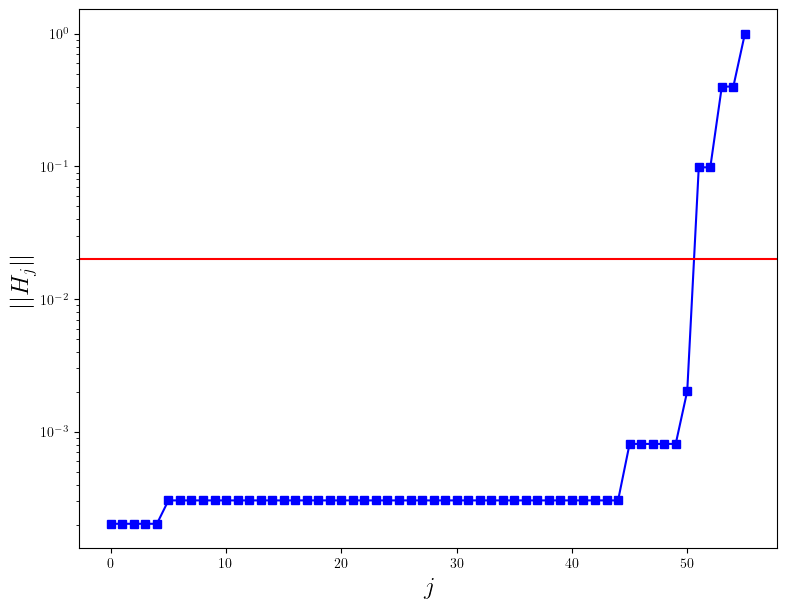
\includegraphics[width=1\textwidth]{composite_numerics/J5dist.png}
            \caption{}
        \end{subfigure}
        \begin{subfigure}[b]{.49\textwidth}
            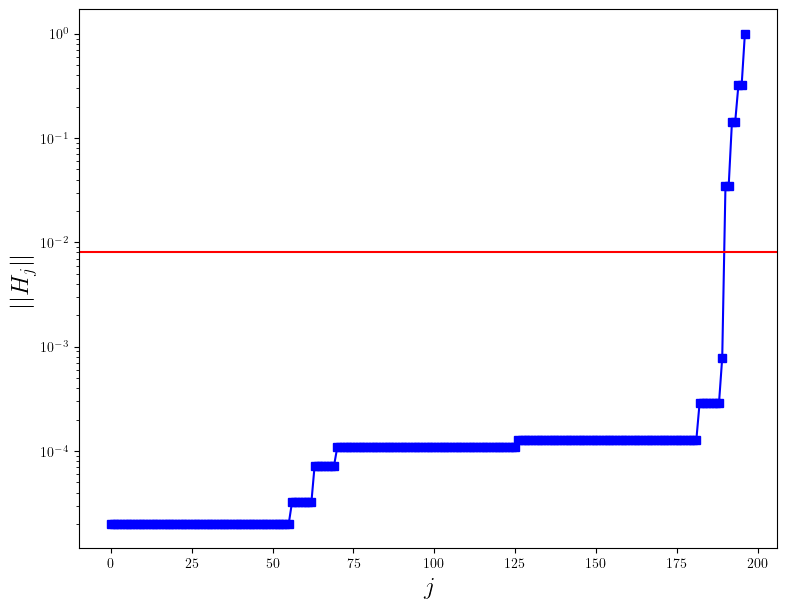
\includegraphics[width=1\textwidth]{composite_numerics/J7dist.png}
            \caption{}
        \end{subfigure}
        \caption{\textit{Jellium Spectral Norm Distribution:} Semi-log plots of the sorted normalized spectral norms versus Hamiltonian index for 5 and 7 site Jellium models in figures (a) and (b) respectively. The plots show the increases in number of terms as well as how the distributions become increasingly sharply peaked. In red we provide a potential choice of $\omega_c$ for the partitioning heuristic.} \label{fig:Jelliumspec}
\end{figure}
\FloatBarrier

\subsubsection{Graph Hamiltonian Model}
The Hamiltonian we explore here involves a spin chain imposed on a lattice $\Gamma \in \mathbb{Z}^D$ with a graph distance metric $dist(\mathbf{u},\mathbf{v}) = |\mathbf{u}-\mathbf{v}|_1$ where $\mathbf{u}$ and $\mathbf{v}$ are vectorized coordinates on the graph with dimension equal to $D$. For our investigation we only examine lattices with $D=1$, given that for a fixed number of sites, this gives the most sharply peaked spectral distribution than any other $D$:

\begin{equation}
    H = \sum_{i>j} e^{-dist(i,j)}\alpha_{ij} \sigma^x_i \sigma^x_j + \sum_k \beta_k \sigma_k^z
\end{equation}

This system is similar to the quantum transverse field Ising model but with interactions that fall of exponentially with graph distance. The coefficients $\alpha_{ij}$ and $\beta_k$ are site dependant coupling constants that allow for the introduction of more disorder and/or structure in the Hamiltonian. To add some disorder to the model, we draw these coefficients pseudo-randomly from a Gaussian distribution with mean 0 and variance 1. \\

\subsubsection{Heisenberg Model}
The Heisenberg model describes a quantum spin system in a magnetic field with nearest-neighbour interactions. The Hamiltonian takes the following form:
\begin{equation} \label{eq:heisenberg}
    H = \sum_j \left(J_x \sigma_j^x \sigma_{j+1}^x + J_y \sigma_j^y \sigma_{j+1}^y + J_z \sigma_j^z \sigma_{j+1}^z \right)+ \sum_i B_z \sigma_i^z
\end{equation}
Here $B_z$ is the strength of the magnetic field in the $z$ direction and $J_{\{x, y, z\}}$ are coupling constants. Given the intuition of our composite channel, we expect this model to take advantage of our algorithm when the coupling constants largely differ in magnitude such that partitioning into Trotter and QDrift takes advantage of more Hamiltonian structure. Furthermore, introducing site-dependant coupling constants or writing down a highly disordered spin system could further add structure that the algorithm can take advantage of. A Hamiltonian of this nature would look something like the following: 
\begin{equation} \label{eq:spin_glass}
    H = \sum_j \left(J_x^{(j)} \sigma_j^x \sigma_{j+1}^x + J_y^{(j)} \sigma_j^y \sigma_{j+1}^y + J_z^{(j)} \sigma_j^z \sigma_{j+1}^z \right) + \sum_i B_z \sigma_i^z
\end{equation}
This Hamiltonian appears somewhat contrived for extracting the performance of the local composite channel. However, this system closely resembles the Edwards-Anderson model of a spin glass, a system of interest in condensed matter physics. In an attempt to create a sharp distribution, we simply sample $J_\nu^{(j)}$ from an exponential distribution with a scale parameter of 0.1. \\

\subsection{Partitioning Schemes} \label{sec:partition_scheme}
The main difficulty with deploying the composite simulation framework concerns  finding a good partitioning. In introducing composite simulations, Hagan and Wiebe suggested partitioning schemes derived on the basis of optimizing analytic cost functions both in deterministic and probabilistic settings \cite{hagan2022composite}. Here, we take a different approach involving the exact calculation of the simulation error, and an optimization routine that, given convergence, finds the optimal partitioning and gate count with respect to a chosen error tolerance and simulation time. This approach is used to answer the question regarding the best savings one can hope to achieve when deploying composite methods to simulate a specific Hamiltonian. We are not proposing this as a pre-processing routine (for a study of this nature see Ref. \cite{mc2023classically}), as it has complexity greater than that of the simulation itself, which is trivial as the optimization involves solving the simulation problem recursively. In addition, we also arrive at simple heuristics that can be used to partition certain Hamiltonians with little overhead, which we do propose as a strategy for using a composite approach. \\

\textit{Chop} is the partition that we introduce in this work. The idea is based on the heuristic of placing a few terms with larger spectral norms into Trotter-Suzuki channels and numerous small terms into QDrift, assuming that the Hamiltonian presents this structure. We start by sorting the terms by their spectral weights and introducing a ``chop threshold" $\omega_c \in [0, \max_i h_i]$. This scale will determine the partition such that if a term has spectral norm $h_i\geq\omega_c$ then $H_i\rightarrow A$ if $h_i < \omega_c$ then $H_i\rightarrow B$. Now we can express the error tolerance $\epsilon$ as a function of channel iterations $r$, with partitioning chop $\omega_c$ and a sample number $N_b$ that will be chosen in an optimization routine, and for a fixed initial state and time:
\begin{equation}\label{eq:errorfunc}
    \norm{(\mathcal{X}^{2k})^{\circ r}(\rho, t/r, \omega_c, N_b) - \evolchan{\rho, t}}_1 = \epsilon(r).
\end{equation}
%
By fixing an error tolerance for $\epsilon$, the exact cost of the simulation becomes a black box function with no closed form expression:
\begin{equation}\label{eq:cost_function}
    C_{comp} = f(\epsilon_{thresh}, r, \omega_c, N_b).
\end{equation}
This is the cost function we wish to minimize. However, we cannot do that by conventional methods such as with direct gradient descent. Also, with no strong intuition for a choice of $N_B$, if we wish to optimize this parameter we have to deal with integer optimization as well. The iterations $r$, however, while an integer, does not require optimization, but rather emits a search problem. If we allow an optimizer to pick initial random values for $N_b$ and $\omega_c$ from a fixed interval, then we must find the value $r$ required to meet the error threshold $\epsilon_{thresh}$, which will ultimately be determined by the optimizer's choice of the other two parameters. To complete this, we perform an exponential search on $r$ until we find some $r$ where $\epsilon(r) \geq \epsilon_{thresh}$ and set this as an upper bound on $r$. We then perform a binary search to find the smallest value of $r$ required to meet this condition and count the number of gates in the channel. This is a very expensive function given that we are precisely building the composite channel, applying it to the density matrix initial state in the problem, and counting the gates applied in each iteration of the search. The expensive nature emerges due to the sheer number of matrix multiplications required in performing this task, not in the search for $r$, which is nearly optimal. Note the importance of using the trace distance in this approach as it guarantees monotonicity of $\epsilon(r)$, which makes the search possible. This is not so in the framework of sampling the quantum infidelity, as finding the cost here would require other statistical methods (see Appendix \ref{sec:appendix_error}). \\
% DS3 The last sentence is unclear!
%MattP - slight change, and pointed the reader towards where this topic is further discussed.

Now a glaring question left unanswered is the choice of an optimizer. We implement the Gradient-Boosted Regression Trees (GBRT) algorithm included in Sci-Kit Optimize \cite{pedregosa2011scikit}. This algorithm is specifically-designed to handle the optimization of very expensive functions. It is also convenient for our purposes given that it can handle both integer and real optimization parameters simultaneously. At a high level, the algorithm works by using a series of decision trees with an associated loss function. The decision trees perform regression to fit the input function and are iteratively generated based on the minimization of the loss function via gradient descent. This optimizer and cost function \ref{eq:cost_function} can then be easily generalized to the local composite channels where now we have an $N_b$ and $\omega_c$ for each blocking. As the number of local blocks grows, the optimization routine will need to take a larger number of input parameters in this prescription. However, the size of the system becomes classically intractable long before we would consider using this many local blocks, so this is far from a concern. \\

In some cases, models may exhibit a partitioning that is somewhat canonical and can lead to excellent performance of composite methods. This occurs when we have a Hamiltonian that fits naturally into the intuition behind the algorithm, such that we have a set $A$ containing large terms with small commutators and a set $B$ with small terms that are known not to commute in general. We are, therefore, proposing to use the chop partition but by choosing the chop threshold $\omega_c$ based on physical intuition regarding the Hamiltonian, rather than some expensive optimization routine. A perfect example of such a system is a Heisenberg model with weak coupling. In this case, looking at Equation \ref{eq:heisenberg}, we would set the chop threshold $\omega_c = \max\{J_x, J_y, J_z\}$, which implies we simulate the interactions with QDrift $\{J_\nu \sigma_j^\nu \sigma_{j+1}^\nu\}_{\nu = x,y,z} \rightarrow B$, and simulate the site energy terms with Trotter-Suzuki $\{B_z \sigma_j^z\} \rightarrow A$. In this way, the terms in the set $A$ all commute with each other, whereas the terms in the set $B$ are guaranteed to have a small spectral norm. We bring numerical evidence that this provides computational advantages in the sections below. In general, any system with perturbative interactions may benefit from this framework, given that the commutators within the system are small, as they will avail  this canonical partitioning. In cases where the partitioning is not as obvious, as is the case with {\rm H$_3$} and Jellium, we can achieve similar advantages by choosing $\omega_c = \max \frac{d \norm{H_j}}{dj} \textbf{s.t.} \norm{B} \geq \norm{A}$, meaning we sweep an ordered list of the Hamiltonian spectral norms and track the largest difference between terms, chopping the list where this occurs, given $j\geq \frac{L}{2}$. The final condition is just to ensure the majority of terms are simulated by QDrift. We also use this strategy throughout \ref{subsec:performance} and show advantages. 

\subsection{Error Measures} \label{sec:Error_Measure}
In this investigation, there is some arbitrariness in the error measure one can choose in order to quantify the performance of a simulation channel. In order to evaluate the resources required by an algorithm, one must evaluate the number of gates required to meet a certain $\epsilon$, which is calculated by said error measure. In the literature, this $\epsilon$ is often quantified by the diamond distance utilized in previous sections. However, while analytically convenient, for any reasonably-sized system, computing this quantity becomes computationally expensive. While it is possible to evaluate it efficiently, this requires finding the solution of a semi-definite program, which is much less efficient than using some other error measures. In addition, since we are not constrained to analytically solvable expressions or closed form equations with our numerical methods, we can optimize this cost in terms of some partition scheme. This is the idea behind the optimal chop partition, and doing so requires frequent computations of $\epsilon$. With this in mind, the error of our algorithm should be a quantity that we can compute in a reasonable amount of time while also being a fair error measure. The criteria for ``fairness" comes within the error measures treating each algorithm that comprises the composite channel on an equal footing. For example, if we are to optimize the partitioning with respect to the gate cost (which is dependent on $\epsilon$), then if Trotter is more performant with respect to QDrift in one error measure than in another, then our composite optimizer will favor Trotter, which will be reflected in the partition. As a result the total cost of the composite channel will be skewed by the error measure used. \\

We consider the infidelity and trace distance as possible measures of $\epsilon$. For definitions and an additional discussion regarding the scaling and complexity of computing these quantities, see Appendix \ref{sec:appendix_error}. Analytics are required in order to answer the question of which measure might provide a more fair comparison. More specifically, we can ask the question of how the error measures will scale with respect to the total simulation time $t$, and then test these results numerically. In terms of the infidelity, we provide the following Theorems:
\begin{restatable}[QDrift Infidelity Time Scaling]{prop}{qdinfscaling} \label{thm:qdinfscaling}
    Given a QDrift channel $\qdchan{\rho, t}$ and the standard evolutionary channel $\capU(\rho, \frac{t}{N})$, for a density matrix $\rho$, time $t/N$, then the infidelity between the outputs of the channels $1- \fidel(\qdchan{\rho, t}, \capU(\rho, t/N)) \in \bigo{t^2}$.
 \end{restatable}

 \begin{restatable}[Trotter-Suzuki Infidelity Time Scaling]{prop}{TSfidelity} \label{thm:TSfidelity}
Given a Trotter-Suzuki channel $\tschan{2k}{\rho, t}$ and the standard evolutionary channel $\evolchan{\rho, t}$, for a density matrix pure state $\rho$ and time $t$, then the infidelity between the outputs of the channels $1 - \fidel(\tschan{2k}{\rho, t} \capU(\rho, t)) \in \bigo{(t^{2k+1})^2}$.
\end{restatable}

The proofs of these theorems are included in  Appendix \ref{sec:appendix_error}. Here, we obtain the non-trivial result that the infidelity is squared when considering Trotter-Suzuki formulas. This would lead to our optimized chop algorithm to heavily favor this channel over QDrift, and for this reason, we consider it an "unfair" error measure. On the other hand, if we consider how the trace distance scales with simulation time in both algorithms, we obtain the following Theorems:

\begin{restatable}[QDrift Trace Distance Time Scaling]{prop}{QDtracedist} \label{thm:QDtracedist}
Given a QDrift channel $\qdchan{\rho, t}$ and the standard evolutionary channel $\capU(\rho, \frac{t}{N})$, for an arbitrary density matrix $\rho$ and time $t/N$, then the trace distance between the outputs of the channels $\tracedist(\qdchan{\rho, t}, \capU(\rho, t/N)) \in \bigo{t^2}$.
\end{restatable}

\begin{restatable}[Trotter-Suzuki Trace Distance Time Scaling]{prop}{TStracedist} \label{thm:TStracedist}
    Given a Trotter-Suzuki channel $\tschan{2k}{\rho, t}$ and the standard evolutionary channel $\evolchan{\rho, t}$, for an arbitrary density matrix $\rho$ and time $t$, then the trace distance between the outputs of the channels $\tracedist(\tschan{2k}{\rho, t}, \capU(\rho, t)) \in \bigo{t^{2k+1}}$.
\end{restatable}

Here, we see that no such squaring occurs, and the expected time-scaling is obtained. For this reason, we compute the entire density matrix and  $\epsilon$ using the trace distance in all of our numerical simulations. Proofs of the above theorems, as well as further discussions can again be found in Appendix \ref{sec:appendix_error}.

\subsection{Performance Results} \label{subsec:performance}
In this section, we first numerically analyze the real time quantum algorithm given by Hagan and Wiebe \cite{hagan2022composite} and then show equivalent numerical calculations of the imaginary time classical case. To accomplish this, we provide cost plots in which we provide the minimum $C$, or the number of rotation gates to achieve a desired simulation accuracy $\epsilon$ (calculated by the trace distance) for each point in time $t$ or $\beta$. To reiterate, here we exactly compute entire evolution channels with a random initial state $\rho$ sampled from the unit hyper-sphere, and directly apply and count gates. We conclude this section with a brief discussion about numerical studies for the local composite simulation algorithms. In these plots, we study variants of the composite channel and display results with the aforementioned notation with the addition of a tilde over the channel if the partition and $N_B$ have been optimized with GBRT. 
% DS3 Was GBRT defined above? I may have missed that... MattP: yup!
For example, a composite channel with inner-order 2 and outer-order 1 with an optimized partition and number of QDrift samples $N_B$ is written like so $\widetilde{\mathcal{X}}^{2,1}$. Before presenting all of the results, for ease of reference, we find it useful to remind the reader of all relevant notations by summarizing them in the table below:\\
\begin{table}[htbp!] 
    \centering
    \begin{tabular}{| c | c | c | c |}
    \hline
        Notation & Description  \\
        \hline
        $C$ & Algorithmic cost defined in Section \ref{sec:cost_model} \\
        $t$ & Total Simulation time \\
        $\beta$ & Imaginary time/inverse temperature \\
        $r$ & Number of Channel iterations/time-steps \\
        $N_B$ & Number of QDrift samples \\
        $\mathcal{T}^{2k}$ & A Trotter-Suzuki channel of order $2k$  \\
        $\mathcal{Q}$ & A QDrift channel  \\
        $\mathcal{X}^{2k, 2g}$ & A Composite channel with inner-order $2k$ and outer-order $2g$ \\
        $\widetilde{\mathcal{X}}^{2k, 2g}$ & A Composite channel with partition and $N_B$ optimized by the GBRT algorithm \\
        $\mathcal{X}^{2k}_{l=j}$ & A Local Composite channel with inner-order $2k$ and block length $l=j$ \\
        \hline
    \end{tabular} 
    \caption{Summary of notation used in the numerical analysis, consistent with previous sections. The channels do not indicate whether we are working in real or imaginary time, however, that will be clear based on the subsections in which plots appear. This will also be the case for local channels simulating Hamiltonians defined on graphs.}
    \label{tab:notation}
\end{table} 

Throughout this section, we normalize $\norm{H} = 1$ and run simulations for times $t \in (0, \frac{3\pi}{2}]$ so as to ensure the system undergoes non-trivial dynamics without overlapping the phase. This is done due to the fact that Trotter formulas have a periodic error for $\norm{H}t\geq 2\pi$, and running simulations in this range would lead to the optimizer finding the ``good points", where the error happens to be small, which would provide a very low cost simulation and a sharp drop in the cost trend. We also report the cost advantages achieved on \textit{crossover points}, which are values of $t=t'$ such that $C_{QD}(t') = C_{TS}(t')$. We denote the composite channel \textit{crossover advantage} as 
\begin{equation} \label{eq:crossover}
    \xi \coloneqq C_{QD}(t') / C_\mathcal{X}(t') = C_{TS}(t') / C_\mathcal{X}(t'). 
\end{equation}
As we are unable to compute these times exactly we use interpolation methods to report values of $\xi$. This is motivated by the fact that analytics suggest this to be the point of greatest advantage for a composite channel \cite{hagan2022composite}. This is intuitive, especially given higher-order Trotter-Suzuki formulas which are known to asymptotically outperform QDrift for large $t$, whilst QDrift is dominant in the small $t$ limit, suggesting a region where their strengths can be combined. Therefore, studying $\xi$ is interesting in that it (given that our optimization scheme is convergent) represents the maximum advantage of using composite simulation algorithms. The value $t'$ at which $\xi$ appears may also suggest time scales for which composite algorithms are most advantageous. However, this analysis does not provide methods for finding $t'$ or predicting $\xi$ a priori as this is a very hard problem. The significance in $t'$ here lies in the fact that we always observe it to fall within the numerical domain of $t||H||\in (0, \frac{3\pi}{2}]$, which coincides with the domain suitable for quantum phase estimation, given we are implementing the real time algorithm. For imaginary time, these values can be viewed as relevant energy-time scales in which these formulas bring a computational benefit, rather than some physically interesting regime. Summarized in Table \ref{tab:numerics_results} are our calculated crossover advantages.

\begin{table}[htbp!]
    \centering
    \begin{tabular}{| c | c | c | c |}
    \hline
        Hamiltonian & $\xi$ & Num. Terms & Time \\
        \hline
        Hydrogen-3 & 2.3 & 62 & Real \\
        5 Site Jellium & 9.2 & 56 & Real \\
        6 Site Jellium & 18.8 & 94 & Real \\
        7 Site Jellium & 10.4 & 197 & Real \\
        7 Spin Graph & 4.1 & 49 & Real \\
        8 Spin Graph & 3.9 & 64 & Real \\
        \hline
        8 Spin Heisenberg & 3.1 & 29 & Imag. \\
        Hydrogen-3 & 2.3 & 62 & Imag. \\
        6 Site Jellium & 18.8 & 94 & Imag. \\
        \hline
    \end{tabular}
    \caption{Summary of gate cost improvements observed via the \textit{crossover advantage} $\xi$ defined in Equation \ref{eq:crossover} (contingent on optimization convergence). We observe that savings tend to somewhat improve as the number of terms increases (within the same model), with the exception of Jellium 7 where optimizer struggles with partitioning due to the number of terms. This is evident in the lack of monotonicity of $C(\widetilde{\mathcal{X}^1})$ in Figure \ref{fig:Jellium56}. The most significant savings are seen for the Jellium models. Even in cases where the number of terms are comparable to other models, larger advantages are persistent in Jellium. This is further establishes the spectral norm distribution as one of the most important indicators of performance in the composite framework.}
    \label{tab:numerics_results}
\end{table} 
\FloatBarrier

\subsubsection{Real-Time Composite Quantum Simulations}
Beginning with Hydrogen chains, our results are highlighted in Figure \ref{fig:H3}. This plot reveals two interesting features: for long-time simulations, heuristics can be found that essentially match the performance of an optimized formula simply by inspecting the distribution of the norms of individual summands $\norm{H_j}$, and with the optimized routine, we find a significant improvement at the crossover point with $\xi = 2.3$. These plots begin flat for most of the simulation channels, which for the most part, indicates that one application of the channel achieves the desired $\epsilon$ for multiple sequential simulations at small times. This is expected, and is especially common with Trotter-Suzuki formulas, given that with one iteration they apply at least $L$ gates depending on the order, while QDrift provides the option of sampling single gates.

\begin{figure}[htbp!]
    \centering
    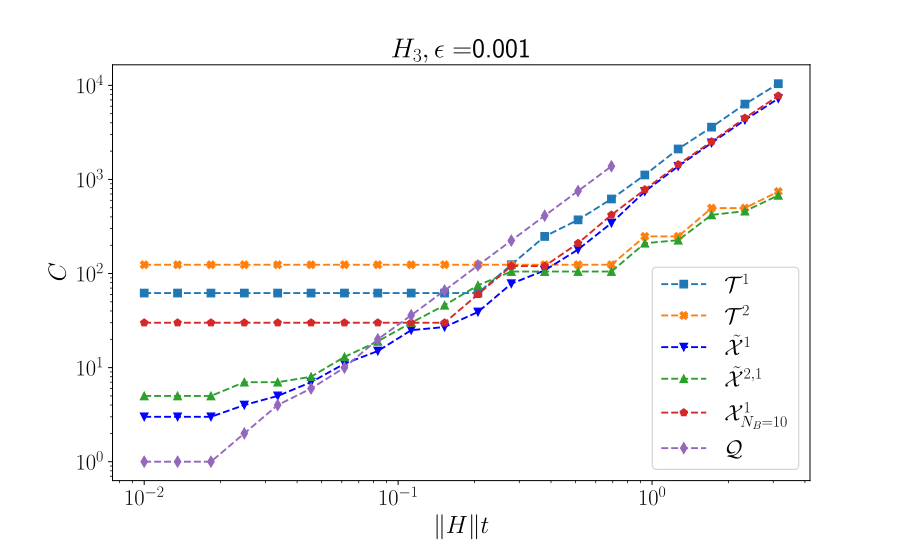
\includegraphics[width=0.6\textwidth]{composite_numerics/H3update.png}
    \caption{\textit{H$_3$ Cost Plot Simulation (Real-Time): }Log-log gate cost plot for the {\rm H$_3$} Hamiltonian generated with OpenFermion using three-dimensional Gaussians in a minimal basis. The bond distance is chosen to be that which minimizes the energy surface of {\rm H$_2$}, which is $\approx 0.8$ angstrom. We achieve a crossover advantage of $\xi = 2.3$, as well as remaining constant factor advantages at long times. For other plot notations see Table \ref{tab:notation}.} \label{fig:H3}
\end{figure} 
\FloatBarrier

Figure \ref{fig:H3} is interesting given that both the heuristic and optimized channels provide significant advantages at the crossover point, as well as the heuristic partition seems to match the asymptotic performance of the optimized channel. This demonstrates that optimization subroutines are not required to gain advantages in this framework. Furthermore, the second inner-order composite channel also shows a consistent advantage over the second-order Trotter channel. \\

To gain insight into effective choices of partition and QDrift samples, we also plot the optimized $N_B$ values and the ratio of Trotter terms to total terms $|A|/|H|$ with time in Figure \ref{fig:H3nbW}. Here, we find choices that somewhat agree with our prior intuition. For short times, places almost all terms into QDrift, and slowly increases $N_B$. As $t$ increases, more terms are placed into Trotter with the partition bouncing around in the regime where Trotter and QDrift have similar costs, which is also expected. The composite channel $\widetilde{\mathcal{X}}^{2,1}$  essentially places all terms into the Trotter simulator, given the favorable asymptotic performance of higher order Trotter formulas over QDrift, while $\widetilde{\mathcal{X}}^{1}$ finds a balance between the two at long times, likely due to their equivalent $t$ scaling. The most interesting behavior is that of $N_B$ at mid to long times. Here, $N_B$ peaks near the crossover point and then falls off as Trotter $t$-scaling becomes dominant in $\widetilde{\mathcal{X}}^{2,1}$. However, for the $\widetilde{\mathcal{X}}^{1}$ channel, $N_B$ experiences somewhat of a revival after the peak, and stabilizes at 15, which is about 24\% of the terms. We use this percentage to motivate future heuristic choices of $N_B$ in our investigation of Jellium in Figure $\ref{fig:Jellium56}$, which turns out to work quite well. 

\begin{figure}[h!] 
    \centering
        \begin{subfigure}[b]{.49\textwidth}
            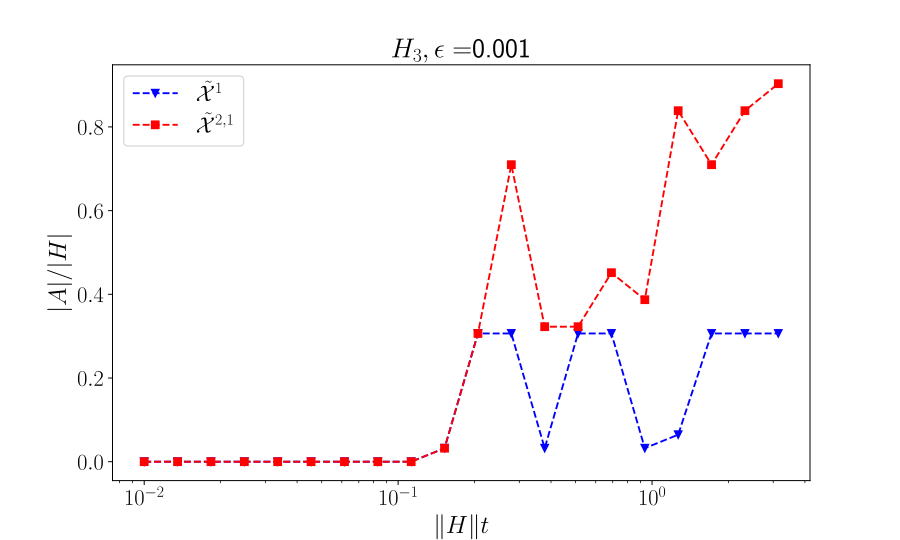
\includegraphics[width=1\textwidth]{composite_numerics/H3_w.png}
            \caption{}
        \end{subfigure}
        \begin{subfigure}[b]{.49\textwidth}
            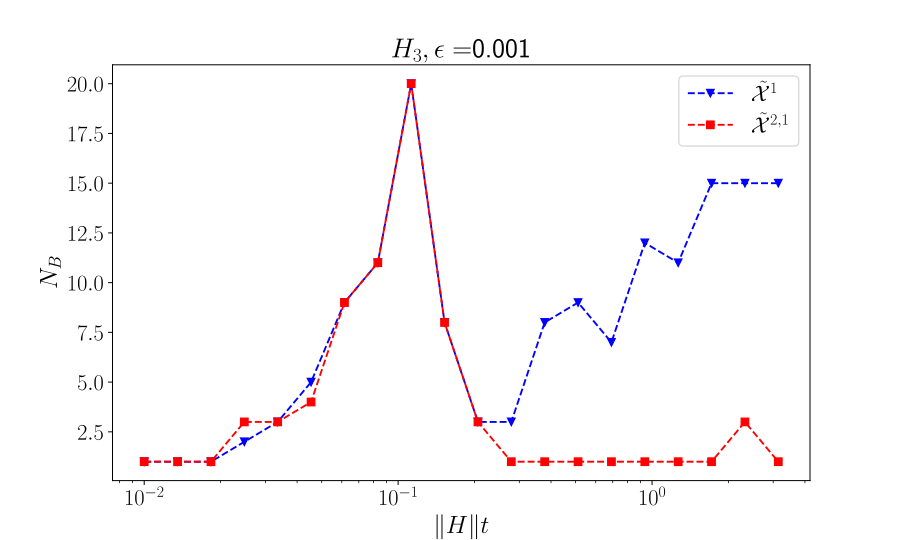
\includegraphics[width=1\textwidth]{composite_numerics/H3_nb.png}
            \caption{}
        \end{subfigure}
        \caption{\textit{Optimized H$_3$ Simulation Parameters:} Semi-log plots of parameters obtained by the GBRT optimization routine for the $\widetilde{\mathcal{X}^{1}}$ and $\widetilde{\mathcal{X}}^{2,1}$ real time channels. These parameter choices correspond to the H$_3$ simulation in Figure \ref{fig:H3}. In (a) we plot the cardinality of the $A$ set over the total number of terms, as a function of time. These values are dictated by GBRT optimized value of $\omega_c$. In (b) we present the equivalent plot with $N_B$. For other plot notations see Table \ref{tab:notation}.} 
        \label{fig:H3nbW}
\end{figure}
\FloatBarrier

When it comes to the simulation of Jellium, we find some of the most significant performance improvements within this section, including an order of magnitude cost difference at the crossover point (see Figure \ref{fig:Jellium56}). Specifically, in the case of 6-site Jellium, the Trotter and QDrift cost at the crossover point is approximately 100 gates, versus the composite channel, which achieves the same precision $\epsilon$ with only about 7 gates. Here, it is also shown that one can find an adequate partition that leads to advantages at longer times without the need for any optimization. This is also the only model whereby the optimization routine struggles to find optimal partitions in the neighbourhood of the crossover point. This leads to the Jellium 7 model inheriting a smaller $\xi$ than what is likely achievable. 
\begin{figure}[h!]
    \centering
        \begin{subfigure}[b]{.49\textwidth}
            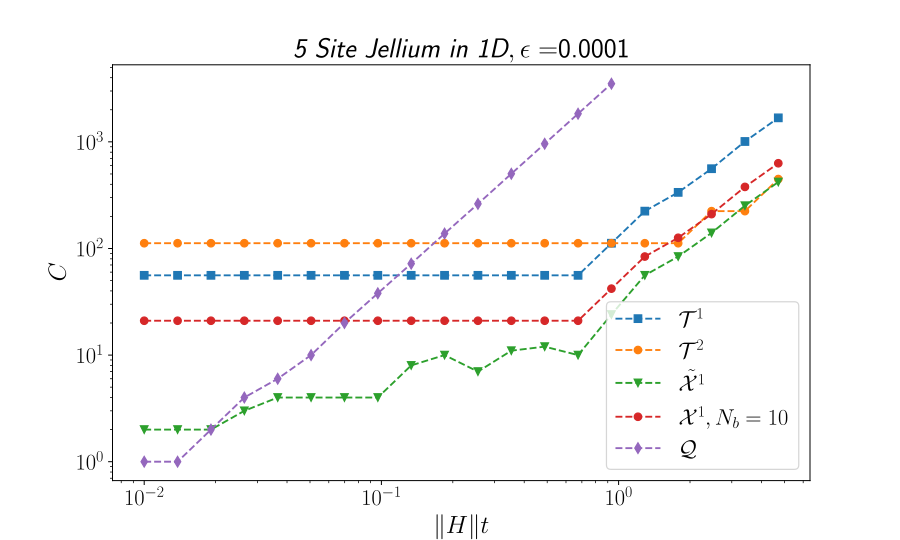
\includegraphics[width=1\textwidth]{composite_numerics/Jellium5.png}
            \caption{}
        \end{subfigure}
        \begin{subfigure}[b]{.49\textwidth}
            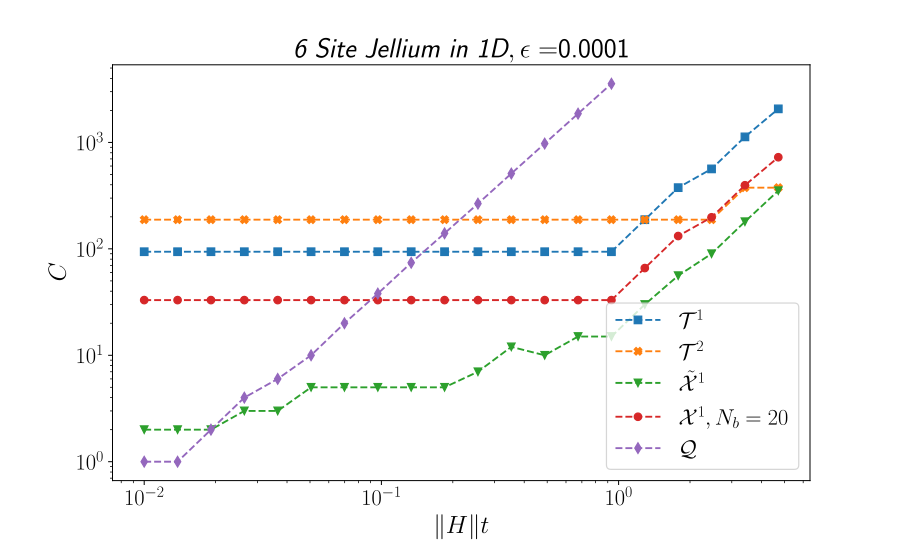
\includegraphics[width=1\textwidth]{composite_numerics/Jellium6.png}
            \caption{}
        \end{subfigure}
        \begin{subfigure}[b]{.49\textwidth}
            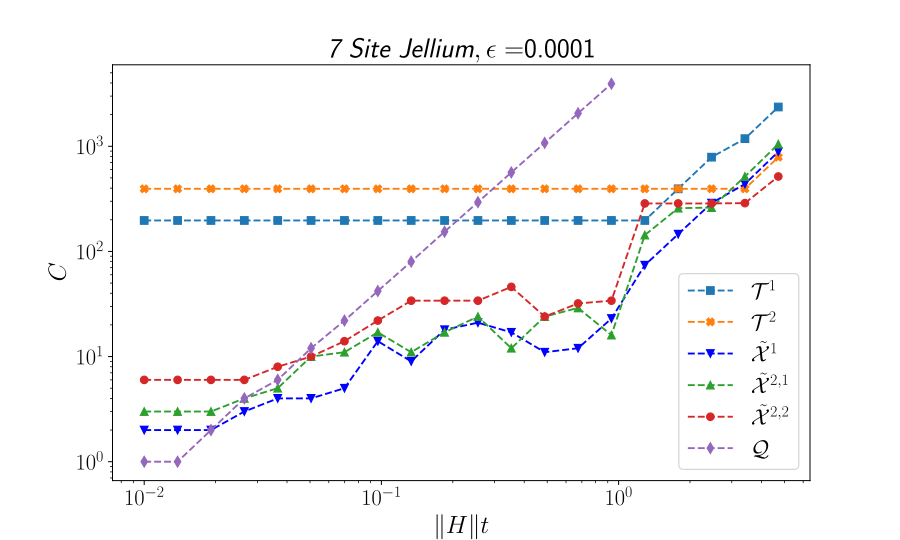
\includegraphics[width=1\textwidth]{composite_numerics/Jellium7.png}
            \caption{}
        \end{subfigure}
        \caption{\textit{Jellium Simulation Cost plots (Real-time): } Log-log cost plots of quantum simulations of Jellium with 5, 6, and 7 sites in (a), (b), and (c) respectively. In (a) and (b) we have in red, a chop heuristic where no optimization overhead is used. The distribution of Hamiltonian terms is chopped immediately before $\max \frac{d \norm{H_j}}{dj}$, and approximately $\frac{1}{5}L$ terms are sampled. This heuristic works quite well, although it is outperformed by the optimized version, especially at short times. In (a) we achieve $\xi = 9.2$. In (b) we achieve an impressive advantage of $\xi =  18.8$, the largest of all our real time results. In (c), we perform a similar analysis of the 7 site model with some higher order composite channels, but find that the optimizer has increased difficulty with larger numbers of Hamiltonian terms. Here $\xi = 10.4$, but through inspecting some neighbouring points of the crossover region, it surely has the potentially to be much larger. For other plot notations see Table \ref{tab:notation}.} \label{fig:Jellium56}
\end{figure}
\FloatBarrier

The final system we investigate in this section is that of the graph toy model with exponentially decaying interactions, which is a beyond nearest neighbour model. In Figure \ref{fig:graph_sim}, we study this model for chains of length 7 and 8, and find essentially identical behaviour. When moving from 7 to 8 spins, we only add 15 more terms to the Hamiltonian, which is clearly not enough to see any significant advantages. In fact, the crossover advantage is slightly smaller for the bigger model, but this could also be due to the optimizer not fully converging. 

\begin{figure}[htbp!]
\centering
    \begin{subfigure}[b]{.49\textwidth}
        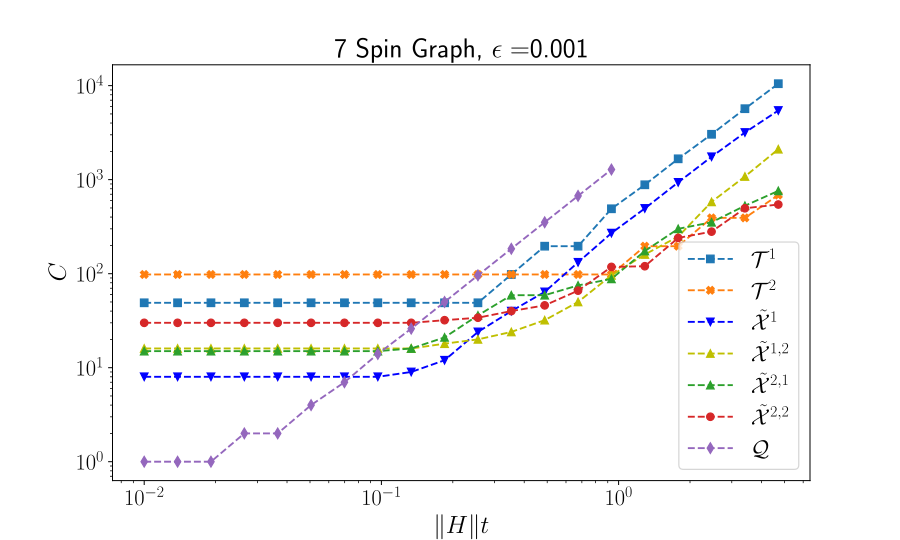
\includegraphics[width=1\textwidth]{composite_numerics/graph7.png}
        \caption{} 
    \end{subfigure}
    \begin{subfigure}[b]{.49\textwidth}
        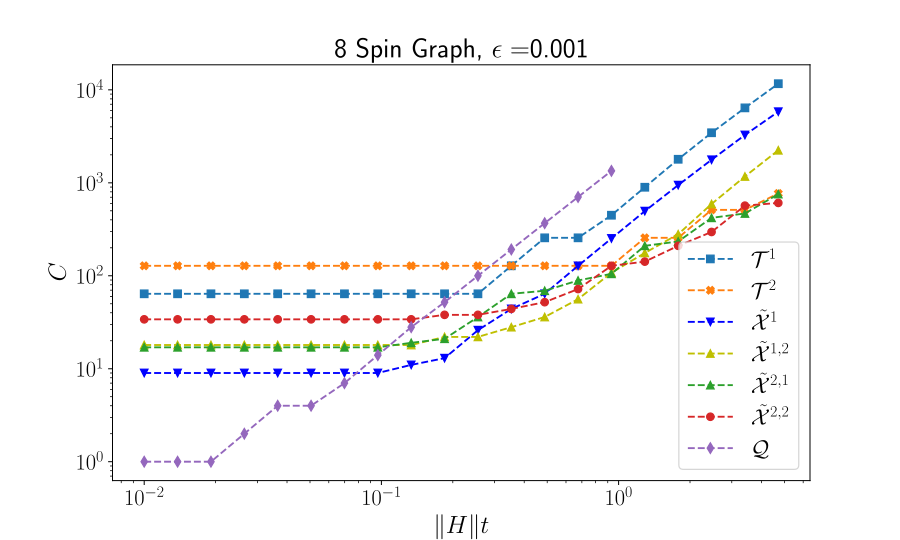
\includegraphics[width=1\textwidth]{composite_numerics/graph8.png}
        \caption{} 
    \end{subfigure}
    \caption{\textit{Toy Spin Graph Model Cost Plot:} In (a) the we have a cost plot for the 7 spin model where we obtain a crossover advantage of $\xi = 4.1$, which is fairly significant. The plot has multiple regions where different composite channels are optimal. In (b) we have the 8 spin model where we establish $\xi = 3.9$. This advantage, as well as the channel performance is almost identical to (a). For other plot notations see Table \ref{tab:notation}.}
    \label{fig:graph_sim}
\end{figure} 
\FloatBarrier

\subsubsection{Imaginary-Time Composite Channels} \label{subsubsec:iTime_results}
This section contains cost plots of simulations of the same aforementioned Hamiltonians, but with imaginary time propagators, where we present cost plots of the most interesting Hamiltonians from the previous section.\\

For simulations of the Heisenberg model, we find similar advantages to those in real time. In Figure \ref{fig:imag_sim}, we see that our proposed heuristic leads to an advantage over Trotter-Suzuki and QDrift in the regions of interest. What is different about this plot is that the optimizer finds the same $N_B$ and partitioning for all short times. This is an artefact of both the Hamiltonian and how the optimizer is programmed. Since all the splitting (single site) terms have equal spectral norm, the optimizer is placed in an all or nothing scenario, as choosing $\omega_c < 1$ immediately places all terms into QDrift. Given that after receiving the cost, the program then solves a search problem to find the minimal $r$ to achieve $\epsilon$ precision, it is rare that it finds the ideal conditions to build a pure QDrift channel with $r=1$. However, significant savings are still achieved at the crossover point, and over $\mathcal{T}^1$ and $\mathcal{T}^2$ at large $\beta$. Once again, the validity of heuristic partitions are shown, specifically in the 1st order composite channel, which exactly matches its optimized version at large $\beta$. \\

\begin{figure}[htbp!]
    \centering
    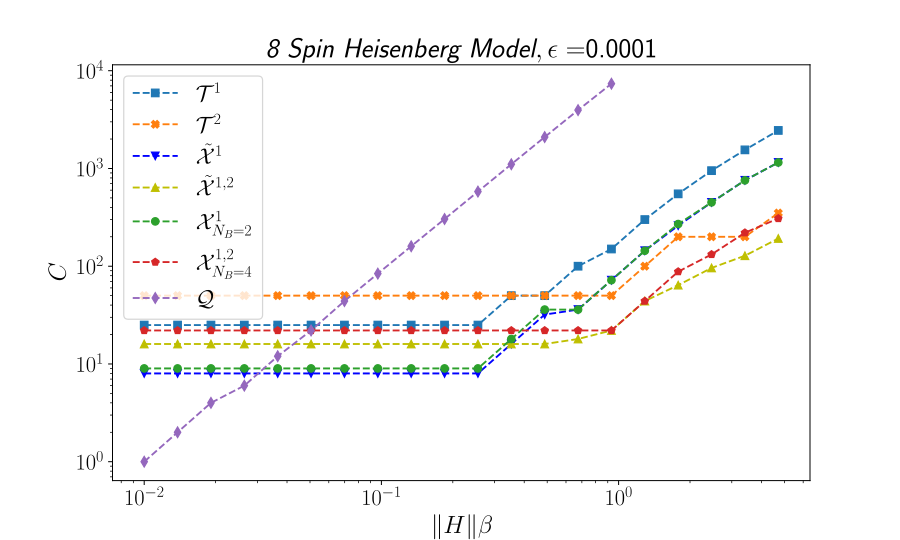
\includegraphics[width=0.7\textwidth]{composite_numerics/iHeisenberg8.png}
    \caption{\textit{8 Spin Heisenberg Model Cost Plot:} In this imaginary time simulation we establish $\xi = 3.1$, as well as maintain advantages at large $\beta$. We also find that our chosen heuristics are essentially optimal at large $\beta$, with the green and dark blue lines overlapping. For other plot notations see Table \ref{tab:notation}.} \label{fig:imag_sim}
\end{figure} 
\FloatBarrier


For Hydrogen chains, we obtain strikingly similar results and compared with those in real time, as seen in Figure \ref{fig:iH3}. We once again obtain a significant crossover advantage, as well as constant factor advantages at large $\beta$, or low temperature. Heuristics are also shown to continue to hold in their effectiveness, in this case, from the crossover point and onward.

\begin{figure}[htbp!]
    \centering
    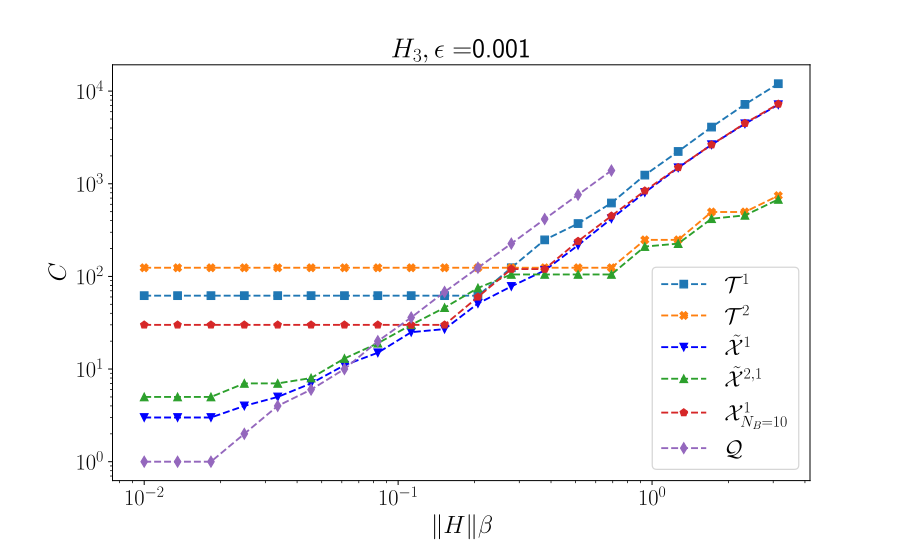
\includegraphics[width=0.7\textwidth]{composite_numerics/iH3.png}
    \caption{\textit{H$_3$ Simulation Cost Plot (Imaginary-Time):} The same parameters are used to build the 3 atom Hydrogen chain as we done in real time. We achieve incredibly similar results, and again recover the real time result of $\xi = 2.3$ that was achieved in Figure \ref{fig:H3}. For other plot notations see Table \ref{tab:notation}.} \label{fig:iH3}
\end{figure} 
\FloatBarrier

For Jellium, we choose to investigate the system size with the best-behaved optimizer, as well as the largest $\xi$, which occurs for the 6-site model. In imaginary time, we once again reproduce a significant advantage, shown in Figure \ref{fig:iJellium6}. As in the case with {\rm H$_3$}, this plot is quite similar to the real time case in Figure \ref{fig:Jellium56}. However, here at large $\beta$ the composite channel seems to do better in imaginary time given that even the first order composite channel (with optimization) outperforms the second order Trotter channel. This happens in the final point of the plot where $\mathcal{T}^2$ is no longer in the``flat-regime". While this is very interesting, it is unclear analytically why this occurs, and we would likely not expect this trend to continue asymptotically. 

\begin{figure}[htbp!]
    \centering
    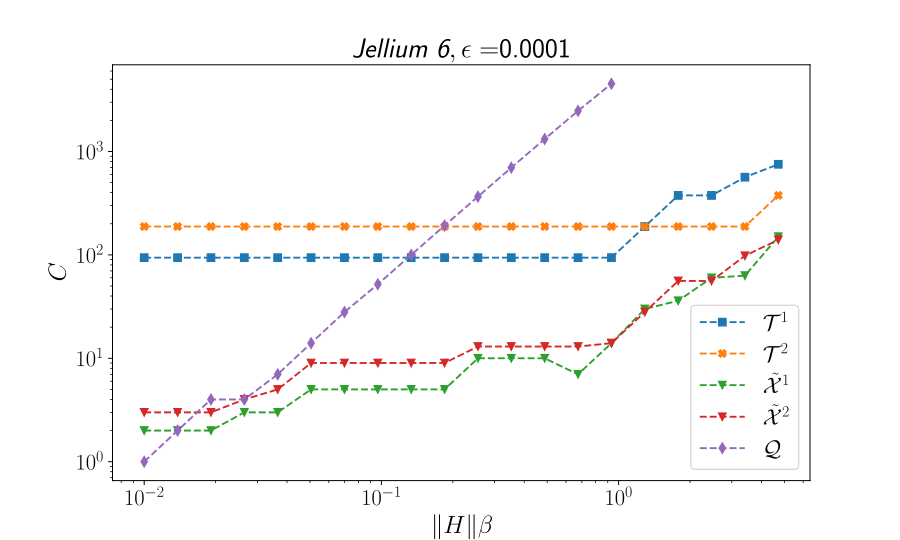
\includegraphics[width=0.7\textwidth]{composite_numerics/iJellium6.png}
    \caption{\textit{6 Site Jellium Simulation Cost Plot (Imaginary-Time):} Here we recover the  crossover advantage of $\xi = 18.8$ from the real time simulation in Figure \ref{fig:Jellium56}, which is also the largest advantage achieved in our imaginary time simulations. We additionally achieve advantages over second order Trotter at large $\beta$. For other plot notations see Table \ref{tab:notation}.} \label{fig:iJellium6}
\end{figure} 
\FloatBarrier

Overall, this section nicely complements some of the analytics in Section \ref{sec:analysis} both by reinforcing the fact that composite quantum channels allow for similar advantages in both real and imaginary time, as well as through calculation of exact constant factor advantages. In other words, this section provides convincing evidence on the applicability of composite formulas to classical imaginary-time Monte-Carlo algorithms.


\subsubsection{Local Composite Quantum Channels}
Distinct from the previous two algorithms, with the local composite channels we do not immediately expect to see significant simulation advantages for the small systems we can compute. Recall, this algorithm makes use of the Lieb-Robinson velocity $v_{LR}$ that limits the propagation of information and thus correlations in a local lattice model. In our above numerics, our lattices contain $\leq 8$ sites, meaning even for small $v_{LR}$, the lattice can still become quickly entangled. In this section, it is important to understand where the observed advantages are originating, whether they are from the local decomposition, or something else. For example, the results in prior sections already suggest that composite channels can outperform Trotter and QDrift channels in certain regimes. If a block decomposition is introduced, we pay a small gate cost to break the simulation into subsets (as gates on the boundary are applied more than once), but the advantages of the composite simulation are almost guaranteed to outweigh this cost. Thus we wish to find a regime in which we can perform calculations of exact costs with local composite channels that explicitly gain advantages via block decomposition. Otherwise, we will observe essentially the same behaviour as before, but with slightly smaller constant factors. There are two ways to go about achieving this; one is to add more sites to the model, which quickly becomes computationally intractable with standard methods. The second strategy is to decrease the coupling between sites in the lattice, which naturally decreases $v_{LR}$. This is the strategy we utilize. In reference to Equation \ref{eq:heisenberg} we perform our cost plots on Heisenberg models with 8 sites with $B_z = 1$, and $J_\nu^{(j)}$ sampled from an exponential distribution with a scale parameter (serving as a coupling constant) of 0.00005. To allow for a fair simulation, we then choose $\epsilon = 0.000001$, such that statistically, $~98\% $ of terms will be greater than $\epsilon$, which can be seen from a simple integration of the PDF. Results of this simulation are shown in Figure \ref{fig:local_heisen}.  \\

\begin{figure}[htbp!]
    \centering
    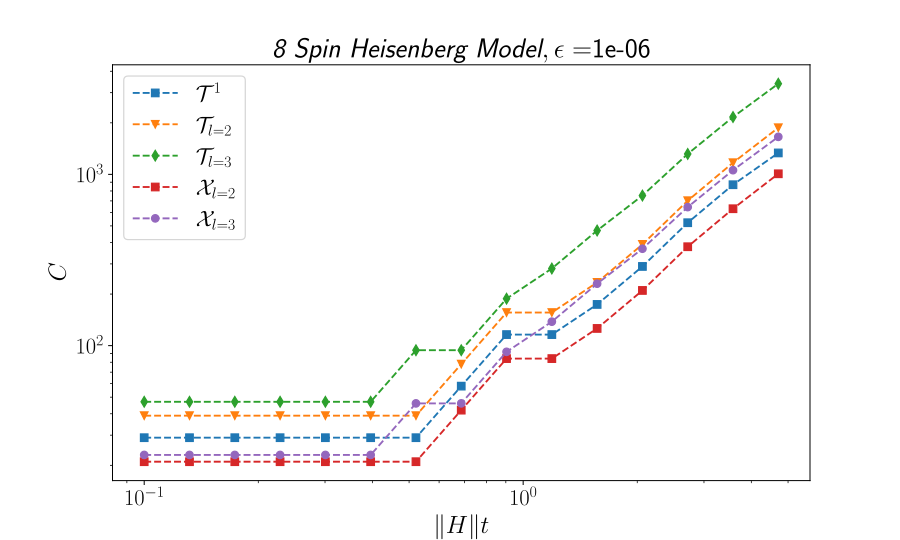
\includegraphics[width=0.7\textwidth]{composite_numerics/local_Heisen8.png}
    \caption{\textit{8 Spin Heisenberg Model Simulated by localized and standard channels:} This cost plot compares Trotter to its  localized versions, with the subscript $l$ indicating the overlap of the boundary region in the block-local simulation.  Channels with no $l$ subscript are the standard simulations from prior sections. As expected, we observe that the composite channel is most efficient, however, given that the standard Trotter algorithm outperforms the localized Trotter channel, we can conclude that we are not in the regime where locality is providing advantages. The same heuristics were used for the composite channel as in Figure \ref{fig:imag_sim}, with $N_B = (4,1,4)$ on lattice subsets $(A, Y, B)$. For other plot notations see Table \ref{tab:notation}.} \label{fig:local_heisen}
\end{figure} 
\FloatBarrier

Given the gap between $\mathcal{T}^1$ and $\mathcal{T}_{l=2}$ in this very weak coupling regime, it is unclear whether our methods (exact gate counts) provide the means for investigating advantages gained by locality. In Ref. \cite{haah2021quantum}, via computations of bounds, numerics did not show advantages (in the form of T-gates) until approximately 100 sites were included in a more strongly-coupled model with $J_\nu^{(j)} \in [-1, 1]$ sampled i.i.d., so our results with far fewer spins are not unexpected. However, we still theoretically expect to see advantages in the limit where system sizes are large, and we can take advantage of the Lieb-Robinson bound.

\section{Thermal State Preparation}

\subsection{Harmonic Oscillator and Single Qubit} \label{sec:specific_numerics}
Now that we have rigorous bounds on each of the parameters $\alpha, t$ and $L$ needed to prepare thermal states of simple systems, we turn to numerics to test these bounds. The first question we explore is how the total simulation time $L \cdot t$ behaves as a function of $\alpha$ and $t$. After, we examine the dependence of the total simulation time on the inverse temperature $\beta$ and we observe a Mpemba-like effect where we find higher temperature states can cool faster than lower temperature ones~\cite{auerbach1995supercooling}. Finally, we demonstrate how our proof techniques could be leading to worse $\epsilon$ scaling than appears numerically necessary. Throughout these experiments we have the same numeric method of starting with the maximally mixed state $\rho_S(0)$ and performing a search on the minimal number of interactions needed for the mean trace distance over all samples to be less than the target $\epsilon$. The number of samples is increased until the variance in the trace distance is less than an order of magnitude below the mean.

In Figure \ref{fig:tot_time_vs_single_time} we explore the total simulation time needed to prepare a thermal state with $\beta = 2.0$ and $\epsilon = 0.05$ for a single qubit system. We plot the total simulation time $L \cdot t$ needed as a function of $t$ for various settings of $\alpha$. We find that increasing both parameters tends to decrease the overall cost until a saturation point is reached, which is at a value of $t$ slightly larger $1/\alpha$. For a fixed value of $\alpha$ this initial decrease in $L \cdot t$ is inverse with $t$, in agreement with our finding of $L \in \bigotilde{t^{-2}}$ in Eq. \eqref{eq:single_qubit_l_bound_2} for $\sigma = 0$. However, this process of decreasing the cost by increasing $t$ can only scale so far and appears to run into a minimum number of interactions $L$ required to thermalize. After this saturation point $L \cdot t$ scales linearly with $t$, indicating that the number of interactions $L$ has reached a minimum. 

Another major take away from Figure \ref{fig:tot_time_vs_single_time} is that it demonstrates that our thermalizing channel is exceptionally robust beyond the weak-coupling expansion in which we can theoretically analyze it. The values of $\alpha t$ used in the far right of the plot completely break our weak-coupling expansion, as we have values of $\widetilde{\alpha}$ that reach up to 500. One interesting phenomenon that we do not have an explanation for is the ``clumping" of various settings of $\alpha$ in the large $t$ limit. As $\alpha t$ dictates the amount of time that the random interaction term $G$ is simulated for, it could be that once a minimum amount of randomness is added via this interaction it is no longer beneficial in causing transitions among system eigenstates. 

\begin{figure} 
    \centering
    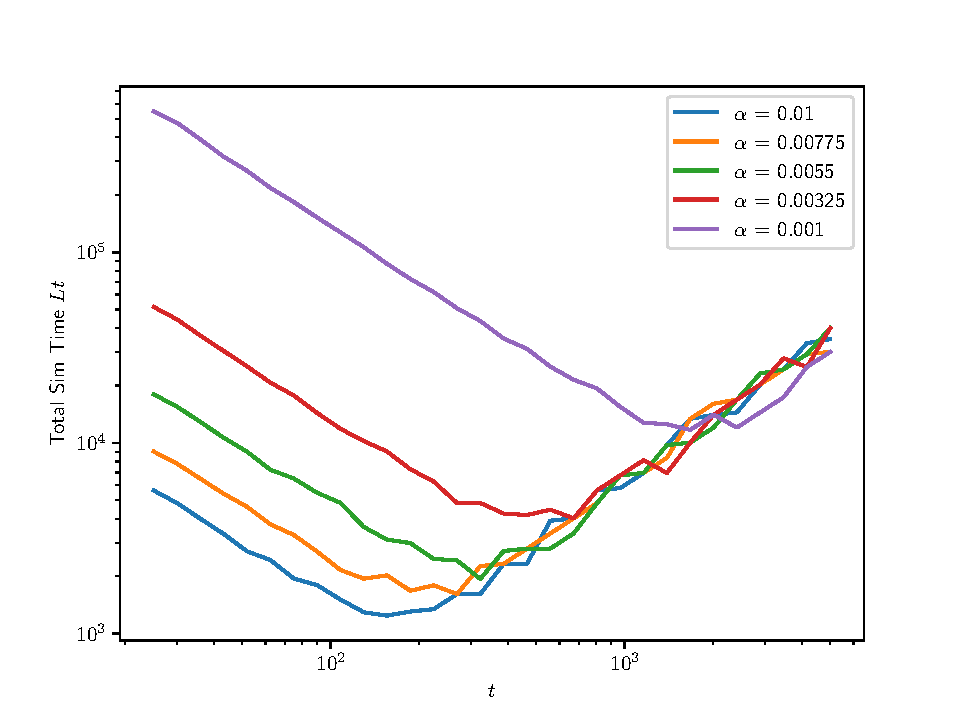
\includegraphics[width=0.75\linewidth]{tsp_numerics/data/single_qubit_tot_time_vs_t.pdf}
    \caption{Total simulation time for a single qubit system to reach within trace distance of $0.05$ of the thermal state for $\beta = 2$ as a function of per-interaction simulation time $t$. The slope of the large $t$ asymptote is $\approx$ 1.01.}\label{fig:tot_time_vs_single_time}
\end{figure}

The next task we have is to examine the $\beta$ dependence. For the harmonic oscillator Theorem \ref{thm:harmonic_oscillator} is helpful for giving an idea of the total simulation time for the ground state but we cannot extend it to finite $\beta$ due to the special structure of the transition matrix in the $\beta \to \infty$ limit. Perturbation theory could possibly be used to extend the computation of the spectral gap to the low temperature regime, but even then it would break down for large temperature (small $\beta$). For generic $\beta$ the structure of the harmonic oscillator transition matrix is tridiagonal but it is not quite Toeplitz, as the main diagonals deviate in the upper left and bottom right corners. We could try to pull these deviations into a separate matrix and treat them as perturbations to a fully Toeplitz matrix, which we can then compute the spectrum of. The issue with this approach is that these deviations are on the order of $\widetilde{\alpha}^2 q(0)$ and $\widetilde{\alpha}^2 q(1)$, which are comparable to the eigenvalues of the unperturbed matrix.

In Figure \ref{fig:sho_total_time_vs_beta} we are able to probe the total simulation time and spectral gap of the harmonic oscillator as a function of $\beta$. We reveal a rather surprising Mpemba-like phenomenon where it takes longer for an infinite temperature initial state (the maximally mixed state) to cool to intermediate temperatures than low temperature states. The Mpemba effect \cite{mpemba} is a classical phenomenon related to the time needed to freeze hot water compared to room temperature water with mentions going all the way back to Aristotle. This phenomenon has been extended to quantum thermodynamics and observed in both theory \cite{nickMpemba}, \cite{mpembaExplanation} and in recent experimental research \cite{zhang2025mpembaObservation}. Our observations are not only a further analytic observation, but we are able to provide a proposed mechanism that explains the behavior. It is clear that the distance of our initial state to the target thermal state $\norm{\rho_S(\beta) - \rho_S(\infty)}_1$ increases monotonically with $\beta$ but what is not obvious is that the spectral gap of the underlying Markov chain is \emph{also} increasing. As larger spectral gaps lead to quicker convergences this acts in an opposite way on the total simulation time. The end result is that for small $\beta$ the increase in initial distance is stronger than the increase in the spectral gap and $L \cdot t$ increases. After some amount of $\beta$ these forces flip and the spectral gap effects become stronger than the initial state distance increasing, leading to a reduction in $L \cdot t$. This phenomenon appears to become more pronounced as the dimension of the harmonic oscillator increases, as can be seem in the $\dim_S = 10$ data. Two things remain unclear: the first is what parameters affect the position and height of the peak in total simulation time and the second is if this behavior is present in Hamiltonians with more complicated eigenvalue difference structure than the harmonic oscillator.

\begin{figure}[t]
    \centering
    \begin{subfigure}{0.45\textwidth}
    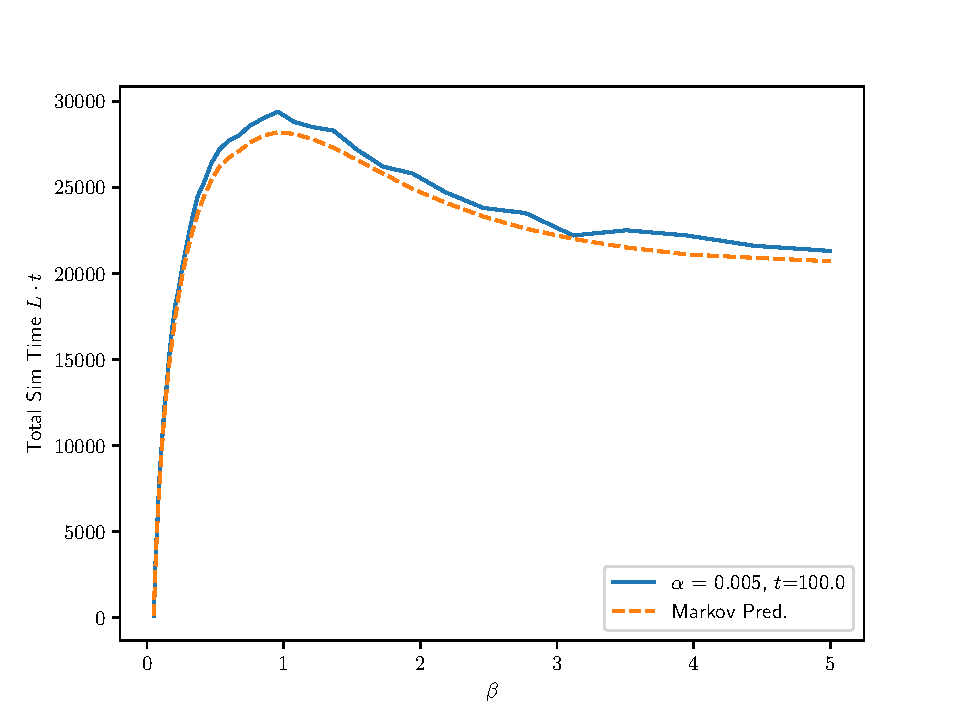
\includegraphics[width=\textwidth]{tsp_numerics/data/sho_total_time_vs_beta_dim_4.pdf}
    \caption{Minimum Interactions vs. $\beta$, $\dim = 4$}
    \label{fig:sho_l_vs_beta_dim_4}
    \end{subfigure}
    \begin{subfigure}{0.45\textwidth}
    \vspace{0.7cm}
    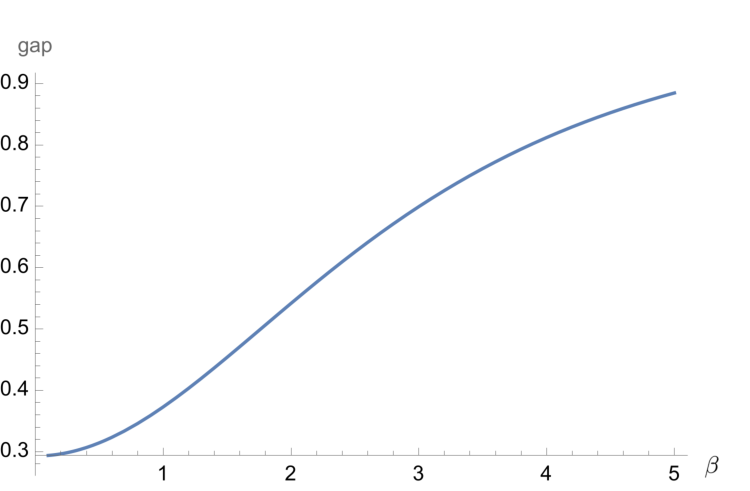
\includegraphics[width=\textwidth]{tsp_numerics/data/spec_gap_dim_4.pdf}
    \caption{Spectral Gap $\widetilde{\lambda}_\star(\beta)$ vs. $\beta$, $\dim = 4$}
    \label{fig:sho_spectral_gap_vs_beta}
    \end{subfigure}
    \hfill
    \begin{subfigure}{0.5\textwidth}
    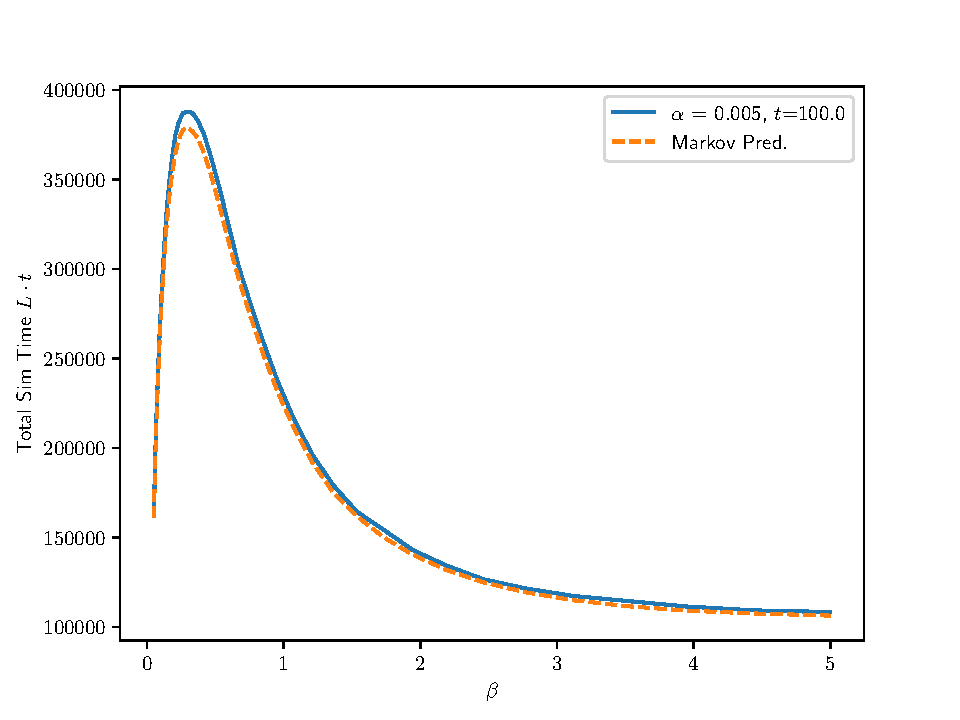
\includegraphics[width=\textwidth]{tsp_numerics/data/sho_total_time_vs_beta_dim_10.pdf}
    \caption{Total simulation time vs. $\beta$, $\dim = 10$}
    \label{fig:sho_l_vs_beta_dim_10}
    \end{subfigure}
    \caption{Demonstration of $\beta$ dependence of the thermalizing channel $\Phi$ for the truncated harmonic oscillator. The environment gap $\gamma$ was tuned to match the system gap $\Delta$ exactly. The minimal number of interactions was found by binary search over values of $L$ that have an average error of less than $\epsilon = 0.05$ with 100 samples.}
    \label{fig:sho_total_time_vs_beta}
\end{figure}

The analytic proofs given in Theorems \ref{thm:single_qubit} and \ref{thm:harmonic_oscillator} are entirely based on our weak-coupling expansion derived in Section \ref{sec:weak_coupling}. The high level picture of this expansion is that we have a remainder error that scales like $\bigo{(\alpha t)^3}$ and an off-resonance error that scales as $\bigo{\alpha^2}$. To balance these two terms we then set $\alpha = \bigo{1/t^3}$. However, as seen in Figure \ref{fig:tot_time_vs_single_time} our thermalization routine appears to be quite robust beyond this weak-coupling expansion, which could lead to significant improvements in runtime. In our derivation for the $\bigo{\alpha}$ and $\bigo{\alpha^2}$ terms we relied on our eigenvalues being I.I.D Gaussian variables, with the first and second order expressions containing factors with the first and second moments respectively of the Gaussian distribution. This would suggest that the third order term in a weak coupling expansion might also be 0, similarly to the first order term. This would lead to a supposed remainder error of $\bigo{\alpha^4 t^4}$, which after balancing with the off-resonance error would give $\alpha = \bigo{1/t^2}$. If the number of interactions then scales like $\bigo{1/\alpha^2 t^2}$, which is consistent with the spectral gap of $\TT_{\on}$ scaling as $\bigo{\alpha^2 t^2}$, then to make the total error of order $\bigo{\epsilon}$ we would require $t \in \bigotilde{1/\epsilon^{0.5}}$ as in Theorems \ref{thm:single_qubit} and \ref{thm:harmonic_oscillator}. This conjecture then leads to a total simulation time of order $\bigo{1/\epsilon^{1.5}}$. 

An even further conjecture would be to keep $\alpha \cdot t$ as a small constant, in this case we are essentially saying that the randomized dynamics $e^{i \alpha t G}$ are beneficial and should not be thought of as some remainder error to be minimized. If the $\alpha t$ constant is small enough then the dynamics will still be approximated by the Markov chain $\TT_{on}$. Our spectral gap will still scale as $\bigo{(\alpha t)^2}$ and $t$ as $\bigo{1/\epsilon^{0.5}}$. This would lead to our total simulation time scaling as $\bigo{1/\epsilon^{0.5}}$. In Figure \ref{fig:epsilon_scaling} we numerically explore these various scalings of $\alpha$ for the harmonic oscillator with $\beta = \dim_S = 4$. Our first remark is that the $\alpha = \bigo{1/t^3}$ scaling as dictated by Theorem \ref{thm:harmonic_oscillator} is numerically supported. 
 Specifically, the theorem suggests that we should observe $O(1/\epsilon^{2.5})$ scaling for $L\cdot t$. 
 Our experiment suggesting $L \cdot t \in \bigo{1/\epsilon^{2.764}}$ which is approximately consistent and deviations from this scaling may arise from the inclusion of data in the fit from outside of the weak coupling limit which is the only regime where we anticipate this scaling. 
 
 We obtained these exponents via least squares fitting of a power-law fit to $L\cdot t$ and $1/\epsilon$. 


\begin{figure}
    \centering
    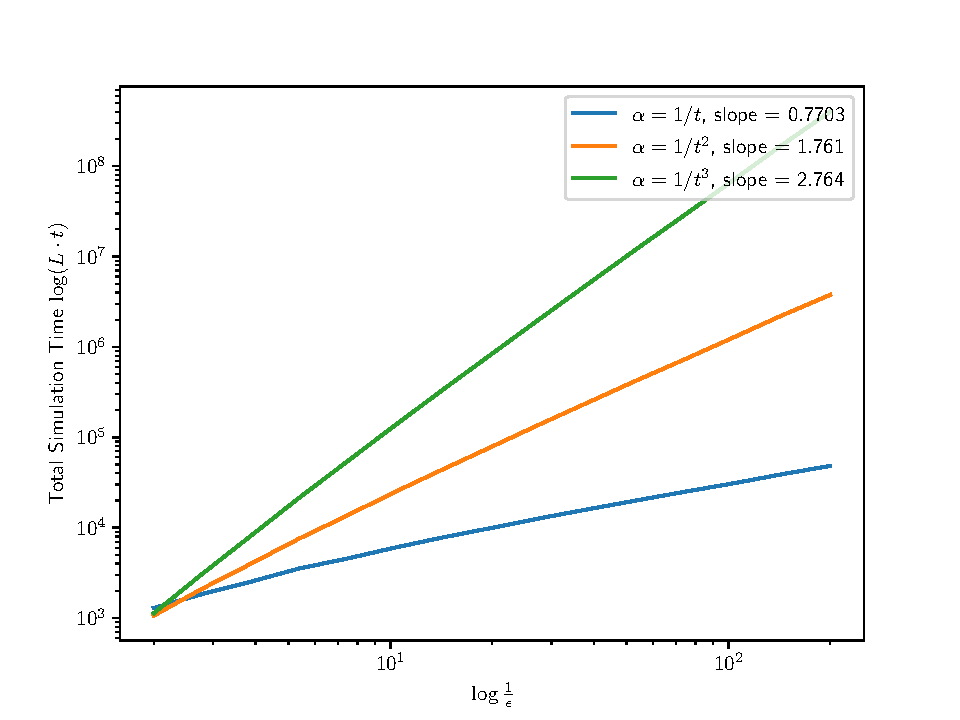
\includegraphics[width=0.66\linewidth]{tsp_numerics/data/epsilon_fitting_4.pdf}
    \caption{Scaling of $L \cdot t$ to prepare a harmonic oscillator thermal state with $\beta = \dim_S = 4$ with respect to $1/\epsilon$ in a log-log plot. For each line in the plot we scaled $\alpha$ by a constant value to make $\widetilde{\alpha}^2 \approx 0.05$ for the largest value of $\epsilon$. Each of these slopes is consistently larger by 0.25-0.27 compared to stated predictions.}
    \label{fig:epsilon_scaling}
\end{figure}



\subsection{Hydrogen Chain Numerics} \label{sec:general_numerics}

The analytic results developed in the previous two sections provide strong guarantees on the correctness of our routine for most quantum systems, however the bounds on the total simulation are fairly high degree polynomials in the parameters of interest. One crucial interpretation of the two different results is that knowledge of the eigenvalue differences of $H_S$ can lead to significantly better simulation time bounds, but this knowledge is not \emph{crucial} for thermalization. Another important takeaway is that we cannot bound the simulation time or number of interactions required for finite $\beta$ as we cannot bound the spectral gap of the expected transition matrix $\EE_\gamma T_\gamma$. The purpose of this section is to investigate these two theoretic takeaways numerically with small Hydrogen chain systems. These systems are some of the smallest chemical systems that still display some real-world chemical behavior, and as a result are typically used in many numeric benchmarks for quantum routines. 

Our first experiment conducted is to study the effects of changing $\alpha$ and $t$ on the trace distance error as a function of $L$. The theory developed in prior sections is very prescriptive; to reach a specific trace distance of $\epsilon$ all of our theorems give a value of $\alpha$, $L$, and $t$ that guarantee a distance of at most $\bigotilde{\epsilon}$ but say nothing about what this convergence looks like. In Figure \ref{fig:h_chain_error} we study the effects of different choices of $\alpha$ and $t$ on this convergence rate. To generate the Hamiltonians used in these experiments we created a small chain of equally spaced hydrogen nuclei with an STO-3G active space for the electrons. Hamiltonian creation was done with OpenFermion \cite{mcclean2020openfermion} and PySCF \cite{pyscf}. Once the Hamiltonians were generated, the distance to the thermal state $\rho_S(\beta)$ for each was tracked over $L = 5000$ interactions. For both Hydrogen 2 and Hydrogen 3 we chose $\beta = 4$ for consistency, this gave a ground state overlap of around 0.56 for Hydrogen 2 and 0.26 for Hydrogen 3. 

\begin{figure}
\centering
    \centering
    \begin{subfigure}{0.49\textwidth}
        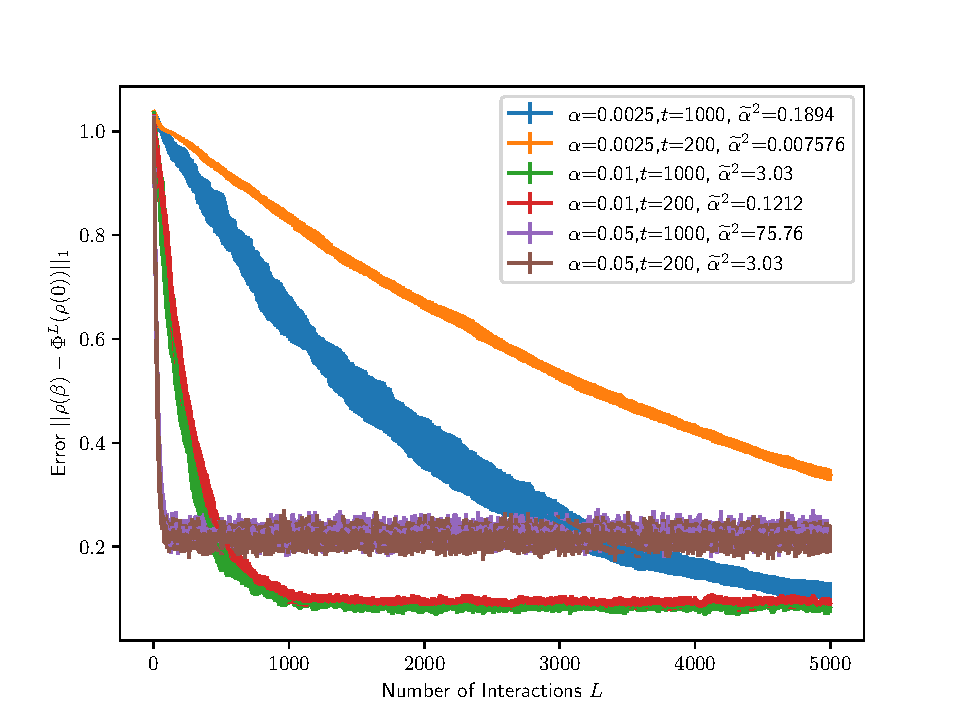
\includegraphics[width = \textwidth]{tsp_numerics/data/error_vs_interaction_h2_chain_1.pdf}    
        \caption{Hydrogen 2 }\label{fig:h2_error}
    \end{subfigure}    
    \begin{subfigure}{0.49\textwidth}
        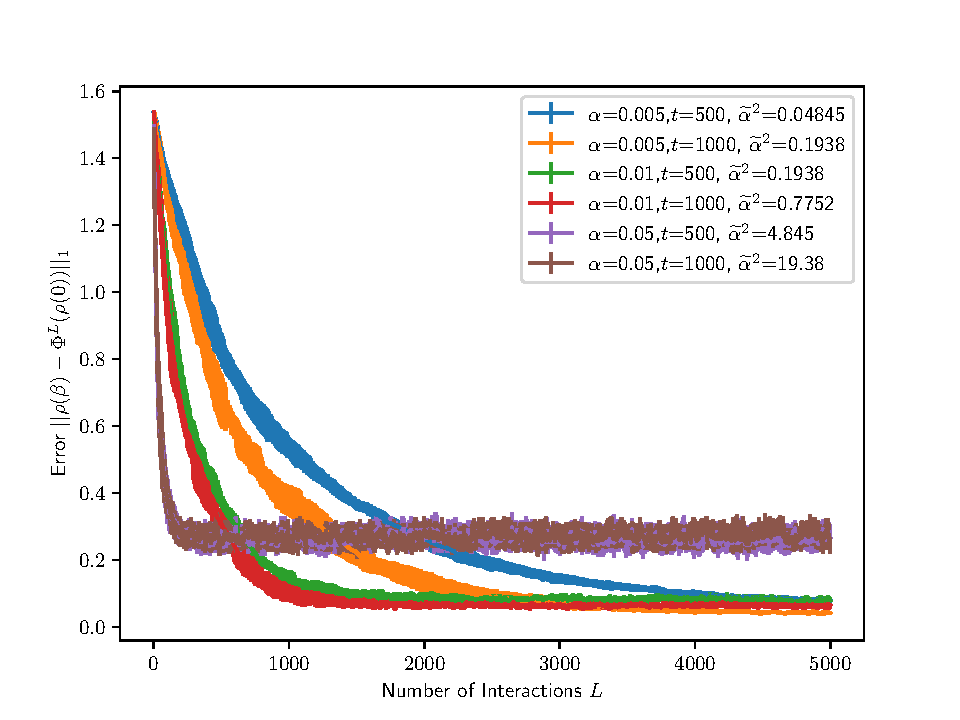
\includegraphics[width=\textwidth]{tsp_numerics/data/error_vs_interaction_h3_chain_3.pdf}
        \caption{Hydrogen 3 }\label{fig:h3_error}
    \end{subfigure} 
    \caption{These plots show the distance to the target thermal state for Hydrogen 2 and Hydrogen 3 chains as the number of interactions $L$ increases. For both Hydrogen 2 and 3 we set $\beta = 4.0$, which gives a ground state overlap of greater than 0.5 for Hydrogen 2 and 0.25 for Hydrogen 3. $\gamma$ for both \ref{fig:h2_error} and \ref{fig:h3_error} was generated by placing a Gaussian at the average energy $\trace{H_S} / \dim_S$ with a width of $\norm{H_S} / 2$. We note that a variety of $\widetilde{\alpha}^2$ values were chosen to demonstrate the faster convergence, but higher error, of strong coupling.
    }
    \label{fig:h_chain_error}
\end{figure}

There are a few key takeaways from Figure \ref{fig:h_chain_error}. The first is that we observe increasing $\alpha$ and $t$ tend to increase the convergence rate, with $\alpha$ visuallly appearing more important. At higher values of $\alpha$ changes in $t$ appear to make less of an impact on the error. We also observe that our channel is seemingly robust beyond our weak-interaction analysis. For values of $\widetilde{\alpha}^2$, the weak-interaction expansion parameter, we observe that values as high as $\widetilde{\alpha}^2 \approx 3$ can have rapid convergence to fairly low error floors. We note that these coupling values that go beyond weak-interaction seem to lead to faster convergence of the dynamics at the cost of a larger error floor. It remains an open question if dynamic choices of $\alpha$ and $t$ could lead to better performance of the overall routine, one could use very large $\widetilde{\alpha}$ initially to quickly thermalize with large error and then decrease $\widetilde{\alpha}$ to fine-tune the final state.

The second observation we make is on the choice of the environment gaps $\gamma$. For both Hydrogen 2 and 3 we selected $\gamma $ randomly from a Gaussian with mean $\trace{H_S} / \dim_S$ and standard deviation of $\norm{H_S} / 2$. This choice of $\gamma$ is completely heuristic and was intended to have a large overlap with what the typical eigenvalue differences may look like with a large enough deviation to pick up potentially large differences. Although this heuristic works well enough to show convergence, it leads us to question if the error convergence or floors can be improved with better choices of $\gamma$. 

In Figure \ref{fig:h_chain_noise} we demonstrate that better choices of $\gamma$ do in fact reduce the total simulation time needed for thermalization. In Figures \ref{fig:h2_chain_with_noise} and \ref{fig:h3_chain_with_noise} we compute the number of interactions needed at a fixed coupling constant $\alpha$ and a fixed time $t$ as a function of the noise added to our samples for $\gamma$. We generate one sample of $\gamma$ by first computing the eigenvalue spectrum of H2 or H3 exactly, then by choosing two non-equal eigenvalues, and finally sampling a Gaussian centered at the absolute value of the difference. The width of this Gaussian then serves as a proxy for the amount of knowledge one may have about the system's eigenvalues. We plot the total simulation time with respect to this width as it varies from 0 to the spectral width $\max_i \lambda_S(i) - \min_j \lambda_S(j)$. The results align well with our theoretic analysis: having knowledge of the eigenvalues of the system can be used to speed up the thermalization routine but if one does not have any knowledge at all the thermal state can still be prepared. It is an open question if the dependence of the total simulation time $L \cdot t$ on the noise level $\sigma$ can be determined analytically.
 \begin{figure}
     \centering
        \begin{subfigure}{0.49\textwidth}
        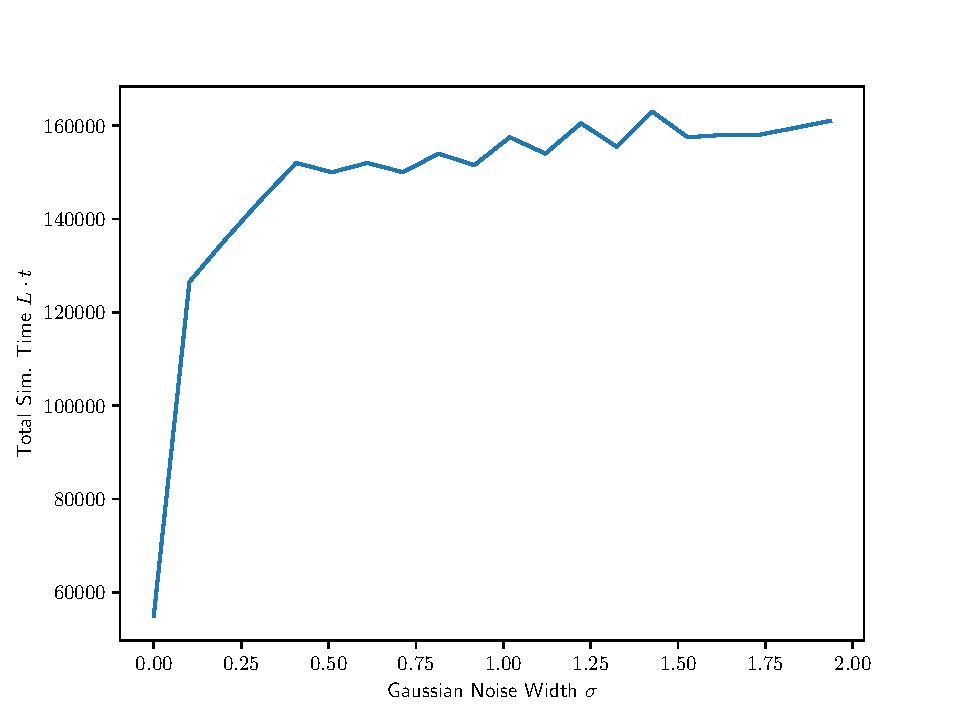
\includegraphics[width = \textwidth]{tsp_numerics/h2_chain_with_noise_3.pdf}    
        \caption{Hydrogen 2 } \label{fig:h2_chain_with_noise}
    \end{subfigure}    
    \begin{subfigure}{0.49\textwidth}
        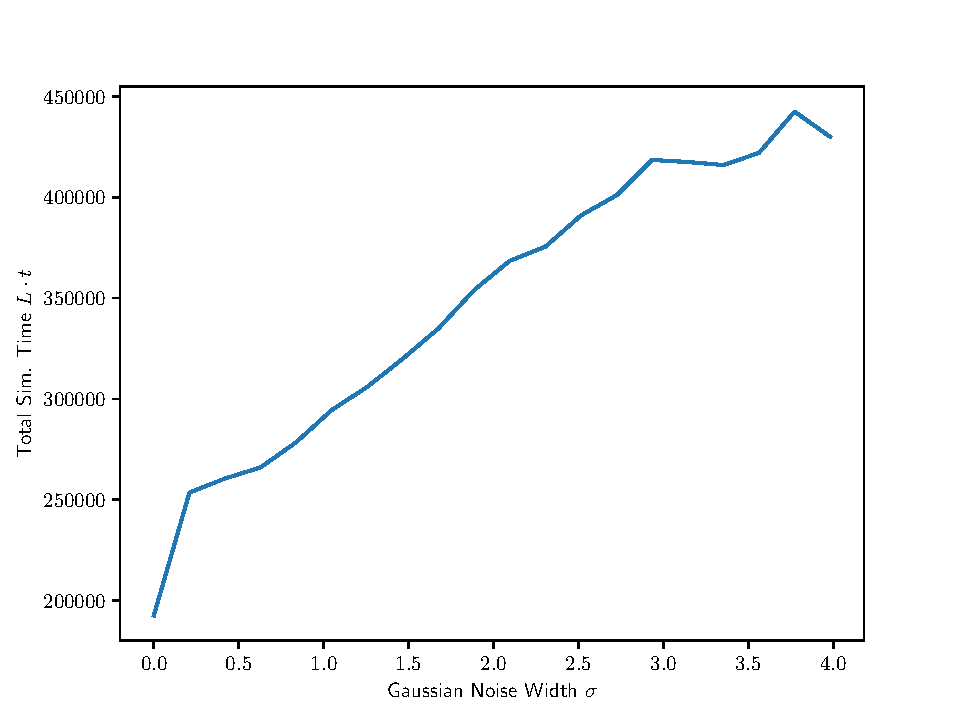
\includegraphics[width=\textwidth]{tsp_numerics/h3_chain_with_noise_3.pdf}
        \caption{Hydrogen 3 }\label{fig:h3_chain_with_noise}
    \end{subfigure} 
     \caption{ In these plots the amount of total simulation time needed to prepare a $\beta = 2.0$ thermal state with $\alpha = 0.01$ and $t = 500$ is tracked as a function of the noise added to samples of $\gamma$. A sample for $\gamma$ is generated by choosing two non-equal eigenvalues from the system spectrum and adding a Gaussian random variable with standard deviation $\sigma$. For each value of $\sigma$ the resulting state needs to have an average trace distance of less than $0.05$ for 100 samples.}
     \label{fig:h_chain_noise}
 \end{figure}